\chapter{The Lord's Prayer (Part 2: Heaven)}
\vspace{0.6cm}
\begin{center}
\nopagebreak
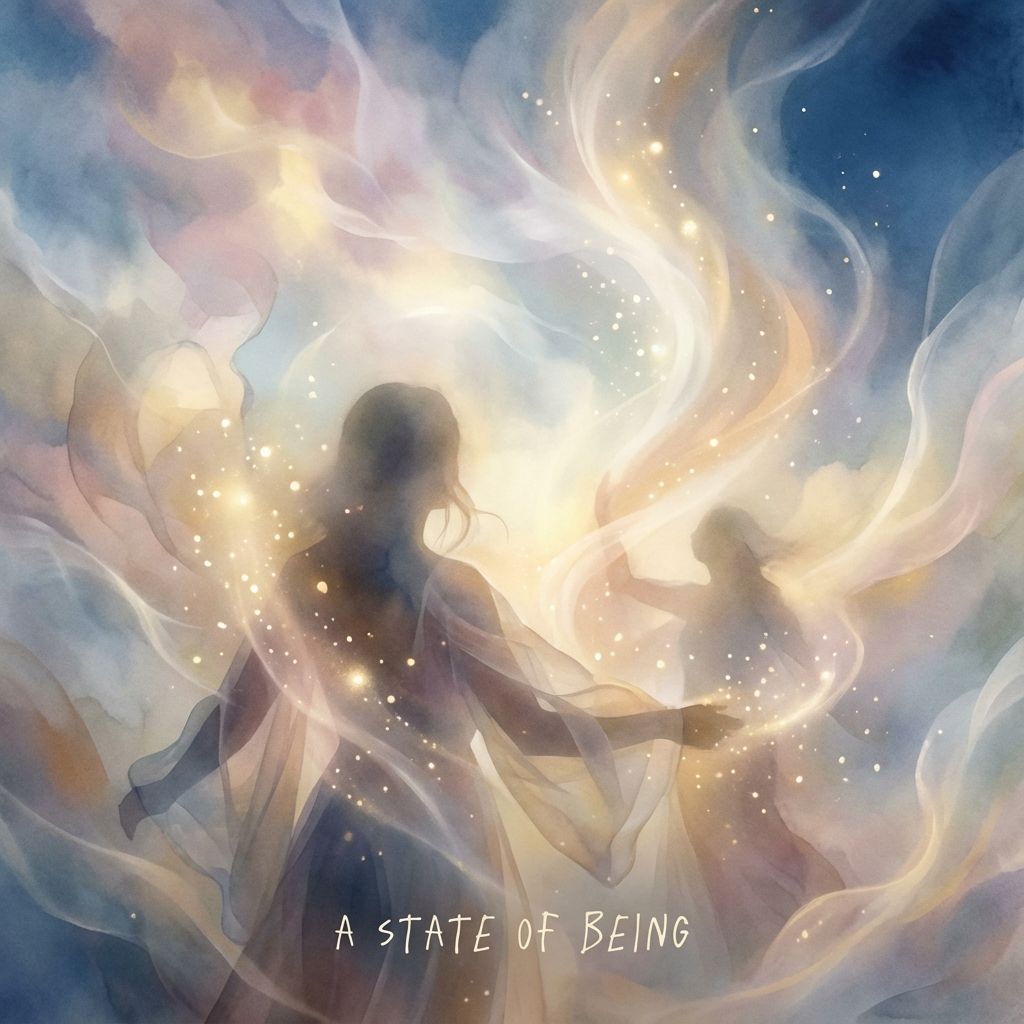
\includegraphics[width=0.75\textwidth,cfbox=gray!60 0.6pt 4pt]{heaven_state.png}\\
\vspace{4pt}
{\small\itshape The Kingdom of Heaven: a wave frequency present here and now.}
\end{center}

\vspace{0.6cm}
Walking down Gran Vía again, surrounded by glowing advertisements and people with shopping bags, Jesus pointed upwards.
—``Who art in heaven''. I already told you in Colmenarejo that heaven is a state of consciousness. But I want you to understand something more.


He stopped in front of a luxury shop window.
—People look for heaven here —he pointed to the expensive watches—. They believe that if they have this, they will be happy. That if they get that job, or that partner, they will touch the sky. But heaven is not a place you go to, it is a place you live from.


—How do you live from heaven here, in the middle of traffic and stress?


—By bringing heaven to earth. That is your mission. ``Thy kingdom come''. It's not waiting to die to go to a nice place with clouds. It's making this place, here and now, look like that vibration of love and peace.


—That sounds difficult.


—It is if you try to change the world outside without changing the one inside. If you are at peace, if you vibrate in gratitude, you create a small bubble of heaven around you. And if many do that, the bubbles join together. That's how the Kingdom comes. Not with armies, but with calm hearts.


He looked at me fixedly.
—You are a channel. If you are dirty with fear and resentment, the light doesn't pass. If you clean yourself, if you vibrate high, heaven passes through you and reaches the earth. You are a bridge, Francisco. You all are.